\section{Modeling}
\subsection{IDP}
\subsubsection{Existential Second Order}
The IDP language can express problems that consist of a set of symbols, called the vocabulary $V$, and a theory, called $T$, that uses symbols from this vocabulary.
The symbols in the vocabulary can be propositions, but they can also represent predicates and functions.
These last two types of symbols make the vocabulary, in general, a \emph{second order} object: it is an object that itself \emph{contains} not only propositional symbols, but also first order symbols.
For example, vocabulary V in Listing \ref{lst:vocabularyExample} is a second order vocabulary as it contains the first order symbol \lstinline{Edge/2}.

The theory $T$ is restricted to a \emph{first order} theory, extended with arithmetic, aggregates, and inductive definitions.
An example of such a theory is given in Listing \ref{lst:vocabularyExample}.

Our inference of choice in the graph mining problem is model expansion; we search for an interpretation $I$ of symbols in the vocabulary $V$ such that this interpretation $I$ satisfies the theory $T$.
This corresponds to the implicit \emph{existential quantification} of all symbols in the vocabulary, both the first order as well as the second order symbols.

In conclusion, we say IDP can express model expansion for \emph{Existential Second Order} problems.

\begin{lstlisting}[mathescape,basicstyle=\fontfamily{lmvtt}\selectfont,caption=\ldots, label=lst:vocabularyExample]
Vocabulary V{
    type Node
    p
    q
    Edge(Node, Node)
}
Theory T : V {
    $\forall$n : $\exists$n2[Node] Edge(n,n2) | Edge(n2,n).
    p => q.
}
Structure S : V{
    Node = {1,2,3}
    p
}
\end{lstlisting}
\begin{lstlisting}
Structure Result:V{
    p
    q
    Edge = {1,1;1,2;2,3}
}
\end{lstlisting}


%problems in which there is an existentially quantified, generally second order, vocabulary of symbols and a first order theory with symbols from that vocabulary.
\paragraph{Issue 1}
First, we must represent the set of example graphs, as specified in \textbf{Def.}~\ref{def:gm2}. 
This definition uses a higher order predicate, as shown in \textbf{Listing}~\ref{lst:HOPred}. 
It represents a single graph as a tuple of predicates and functions, visualised in \textbf{fig.}~\ref{fig:LocalCoherence} as the solid shape.
It is clear that this representation is highly locally coherent, and preserves the independence of graph characteristics.
However, as we are restricted to \emph{Existential} Second Order, we cannot express this higher order predicate.

One possible solution is to replicate for each graph the different characteristic predicates and functions, as well as the knowledge (theory) about them, as shown in
in \textbf{Listing}~\ref{lst:multiglobal} and visualised as the dashed shape in \textbf{Fig.}~\ref{fig:LocalCoherence}.
This way of representing the information about graphs is shown in Listing~\ref{lst:multiglobal}.
It is clear that this solution is undesirable due to the way it scales and the editing needed with growing problem instances.
It retains the local coherence and independence of graph characteristics when it comes to data representation, but prohibits the abstraction (generalization) of knowledge about these properties, as evidenced by our obligation to duplicate the theory for each graph.

%GraphInst(E:Node$\times$Node,Lb
\begin{lstlisting}[mathescape,caption=Higher order predicate modeling the set $\graphset{G}$ of Def~\ref{def:gm2}.,label=lst:HOPred]
GraphInst({(1,2),(2,1)},{1$\mapsto$a,2$\mapsto$b},pos).
GraphInst({(1,3),(2,1)},{1$\mapsto$c,2$\mapsto$b,3$\mapsto$a},neg).
\end{lstlisting}
\begin{minipage}[t]{0.5\textwidth}
\begin{lstlisting}[mathescape,caption=Multiple global relations,label=lst:multiglobal]
E1(1,2). lb1(1)=a.
E1(2,1). lb1(2)=b.
E2(1,3). lb2(1)=c.
E2(2,1). lb2(2)=b.
         lb2(3)=a.
\end{lstlisting}
\end{minipage}
\begin{minipage}[t]{0.5\textwidth}
\begin{lstlisting}[mathescape,caption=Indexed global relation,label=lst:indexedglobal]
E(g1,1,2). lb(g1,1)=a.
E(g1,2,1). lb(g1,2)=b.
E(g2,1,3). lb(g2,1)=c.
E(g2,2,1). lb(g2,2)=b.
           lb(g2,3)=a.
\end{lstlisting}
\end{minipage}




A more workable solution is to represent each characteristic property, such as the edge relation, by a single general relation for all graphs, as shown in \textbf{Listing}~\ref{lst:indexedglobal} and by the dotted shape in \textbf{Fig.}~\ref{fig:LocalCoherence}.
This relation behaves the way it should for a specific graph instance based on an additional argument serving as an identifier for the graph of interest.
%This gives rise to a set $G$ of \emph{graph identifiers}, one for each example graph.
This general relation now corresponds to the \emph{disjoint} or \emph{tagged union} of the graphs' relations, where the tags are drawn from a set $G$ consisting of graph identifiers.
It is clear that this representation forces us to give up the local coherence of graph characteristics that was present in \textbf{Def.}~\ref{def:gm2}: 
%Nu kunnen we kijken wat deze truuk doet met onze mogelijkheid om de abstraction van de theory uit te drukken. Normaal mwillen we dit zo schrijven. Hoewel we nu de generalisatie kunnen uitdrukken, verplicht de restrictie tot existentieel s..o ons om de homomorphic mapping functies te tot een globale property te promoveren, hoewel we feitelijk niet geinteresseerd zijn in de concrete mappings. om om te gaan met de afhankelijkheid van deze functies op de spec. vb grafen moeten we... die nu erg lijkt op skolemisation. theory

%Using this trick however, does not influence our ability to 

But can we now express the abstraction (generalization) of knowledge about these properties, such as the positive homomorphic property?
%to separate the constraint describing the positive homomorphic property, and the coint on its number of occurrences.
%This, from a KR point of view, 
%Furthermore, the restriction to ESO requires us 
%As an example, we illustrate this trick by showing on the expression of the positive homomorphic property, where it greatly resembles Skolemization.
As evidenced in \textbf{Def.}~\ref{def:gm2}, normally one would express the positive homomorphic property by quantifying (counting) over all graphs, requiring the existence of a function with the correct properties.
Using this trick, does not influence our ability to express this restriction: Instead of quantifying over the graphs themselves, we can now quantify over the set $G$ of graph identifiers.

\begin{figure}[h]
\centering
\begin{tabular}{l |l l l}
         & $E$ & $l$      & $c$ \\
\hline
$\graph{G}_{1}$  & $E_{1}$ & $l_{1}$ & pos\\
$\graph{G}_{2}$  & $E_{2}$ & $l_{2}$ & pos\\
  \vdots & \vdots  & \vdots  & \vdots\\
$\graph{G}_{n}$  & $E_{n}$ & $l_{n}$ & pos\\
\begin{tikzpicture}[overlay]
  \coordinate (dotted) at ($(1.28,0.2) + (4.8,4)$);
  \coordinate (line) at (7,4.45);
  \coordinate (dashed) at (1.02,1.6);
  \draw [dotted, rounded corners] 
  ($ (dotted) - (4.8,4) $) -- 
  ($ (dotted) - (4.8,1.5)$) -- 
  ($ (dotted) - (5.3,1.5)$) -- 
  ($ (dotted) - (5.3,4)$) -- cycle;
  \draw [rounded corners] 
  ($ (line) - (3.9,2.66)$) --
  ($ (line) - (7.18,2.66)$) --
  ($ (line) - (7.18,3.1)$) -- 
  ($ (line) - (3.9,3.08)$) -- cycle;
  (3.south east) -- (3.south west);
  \draw [dashed, rounded corners] (dashed) circle (3mm);
\end{tikzpicture}
\end{tabular}
\caption{Local coherence\label{fig:LocalCoherence}}
\end{figure}

%These three different ways of representing graphs are summarized in Fig~\ref{fig:LocalCoherence}.

\paragraph{Issue 2}
%Having solved\matthias{circumvented?} our first issue, 
Next, we would like to express the homomorphic property.
This can be done using a count aggregate, as shown in Listing~\ref{QuantifyOutsideVocabulary}.
First we generate the set of all example graphs to whom we can find a homomorphism from our pattern.
We do this by quantifying over all example graphs g or, per \textbf{issue 1}, their identifiers, and subsequently 
expressing the condition under which they are part of this set: i.e. that there must exist a function f that represents a homomorphism from our pattern graph $p$ to $g$.
In principle, we could then proceed by counting the number of elements in this set.

\begin{lstlisting}[mathescape, caption=Quantifying over functions outside the vocabulary, label=QuantifyOutsideVocabulary,basicstyle=\fontfamily{lmvtt}\selectfont]
#{$\forall g$ : $\exists$ $f$ : $f$ is a homomorphism from $p$ to $g$ }
\end{lstlisting}
However, working in IDP, the restriction to ESO forbids us to quantify over first-order entities such as functions outside of the vocabulary.
Thus, we are required to promote the homomorphic mapping functions to a global property in the vocabulary, even though we are only interested in the existence of a mapping, and not in a concrete valid mapping itself.
We prevent the same explosion of mapping functions as with the graph characteristics above, using the same method as above. Note that in this case, it corresponds to Skolemization.
We introduce a general function \verb|f| that represents all homomorphisms, and make its dependency on a specific example graph explicit using an additional argument:
\verb|partial f(graphId, node):node|.
%As it is impossible
%We introduce a general function \verb|f| that represents the homomorphisms, and make its dependency on a specific goal graph explicit using an additional argument:
In Second Order Logic, this dependency would follow directly from the order of the separate quantifications.

We can now use this \verb|partial f| anywhere we would use the regular homomorphic function for a specific graph by fixing the chosen example graph.
Note that this encoding also requires us to make this function \verb|f| partial, as the Graph Mining problem does not require the solution to be homomorphic with \emph{all} example graphs.
%\todo{Of course, other (even uglier) schemes exist to encode this. Should we mention this?}


\paragraph{Issue 3} Much in the same way, limiting ourselves to existential second order prohibits us from expressing the negative constraint on homomorphism (No more than $N_{-}$ negative examples are homomorphic) in the same model.
In fact, the negative constraint asserts a property for all candidate homomorphic functions, which would lead to \emph{universal} quantification.
Therefore, our only recourse is to encode its dual positive constraint and require it to fail when queried.

Take, for example, the pattern candidate and positive and negative example graphs from \textbf{Fig.}~\ref{fig:ex2}.
Assume all nodes have the same label.
With parameters $N_{+}=1$ and $N_{-}=0$, this pattern candidate is clearly an invalid pattern. 
It is homomorphic with both the positive and the negative example.
But because we now look for one general (Skolemized) homomorphic function, we can choose a global which represents a homomorphism with the positive example graph, but not with the negative example graph.
An example of such a solution is shown in Listing~\ref{lst:invalidf}.

ASP, a language family closely related to IDP, can prevent these kind of models by leveraging the minimality property of their models: ASP looks for the minimal answer set models.
By detecting example graphs for which the f does not represent a homomorphism, and %requiring that in this case f must be the total relation
accordingly enlarging the answer set by requiring that in these cases f must be the \emph{total} relation for this graph, the minimality property will cause the solver to look for $f$ that represent a homomorphism for as many example graphs (including negatives) as possible.
This technique, which would allow us the express the negative property in the same model is called the \emph{saturation} technique~\ref{eiter}.
It is clear however that this technique is not derived from a natural KR translation of the Graph Mining definition.
\begin{figure}
  \centering
  \begin{subfigure}[b]{0.3\textwidth}
    \centering
    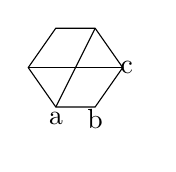
\begin{tikzpicture}[scale=.5]
      \node[circle] at (1,0.7) {a};
      \node[circle] at (2,0.7) {b};
      \node[circle] at (2.8,2) {c};
      \draw (1,1) -- (2,1) -- (2.7,2) -- (2,3) -- (1,3) -- (0.3,2) -- cycle;
      \draw (1,1) -- (2,3);
      \draw (2.7,2) -- (0.3,2);
    \end{tikzpicture}
    \caption{Positive Example}
  \end{subfigure}
  ~
  \begin{subfigure}[b]{0.3\textwidth}
    \centering
    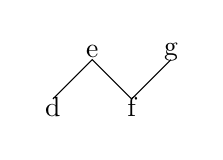
\begin{tikzpicture}[scale=.5]
      \node[circle] at (0,-0.2) {d};
      \node[circle] at (1,1.2) {e};
      \node[circle] at (2,-0.2) {f};
      \node[circle] at (3,1.2) {g};
      \coordinate (1) at (0,0);
      \coordinate (2) at (1,1);
      \coordinate (3) at (2,0);
      \coordinate (4) at (3,1);
      \draw (1) -- (2) -- (3) -- (4);
    \end{tikzpicture}
    \caption{Negative Example}
  \end{subfigure}
  ~
  \begin{subfigure}[b]{0.3\textwidth}
      \centering
      \begin{tikzpicture}[scale=.5]
        \node[circle] at (0.9,2) {1};
        \node[circle] at (2,3.3) {2};
        \node[circle] at (3.15,3.3) {3};
        \draw (1,2) -- (2,3) -- (3,3);
      \end{tikzpicture}
      \caption{Pattern Candidate\label{fig:incorrectcandidate}}
  \end{subfigure}
  \caption{Example 2\label{fig:ex2}}
\end{figure}

\begin{minipage}{\linewidth}
\begin{lstlisting}[mathescape,caption=An possible assignment for f, label=lst:invalidf]
f={
    g1,1$\mapsto$a, g1,2$\mapsto$b,g1,3$\mapsto$c,
    g2,1$\mapsto$a, g2,d$\mapsto$b,g2,e$\mapsto$g
}
\end{lstlisting}
\end{minipage}

%\matthias{Find a convincing but small example}
%\matthias{The moment to introduce the asp saturation technique}

%\paragraph{ASP}
%Let us describe a way to encode the problem into ASP. Conceptually we need to handle three constraints: matching of positive examples, not matching of negative examples and canonicity (that only not isomorphic graphs are produced).

\subsubsection{Inductive Definitions}
Beyond the Existential Second Order restriction, the IDP language is also extended with inductive definitions. These definitions, evaluated under the well-founded semantics, allows the derivation of negative knowledge that otherwise would be underivable.
For example, in \textbf{Fig.}~\ref{fig:trans}, without using inductive definitions, one is unable to derive that point $a$ and $b$ are not connected.
\begin{figure}[h]
    \centering
   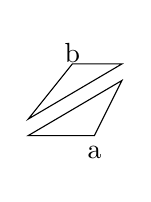
\begin{tikzpicture}[scale=0.7]
   \node[circle] at (2.2,0.7) {a};
      \node[circle] at (1.8,2.5) {b};
       \draw (1,1) -- (2.2,1) -- (2.7,2) -- cycle;
       \draw (1,1.3) -- (1.8,2.3) -- (2.7,2.3) -- cycle;
   \end{tikzpicture}
\end{figure}
%\reversemarginpar
%\todo{A section about inductive definitions, and their use. (Being able to derive negative knowledge)}

\subsection{Faithful encoding}
\matthias{In this subsection, we show a new encoding and argue that it is more faithful to the problem with respect to the definition as given in Def~\ref{def:gm2}.}
\begin{alltt}
  homomorphism(<Edge1, Label1>, <Edge2, Label2>) \(\iff\)
      \big(\(\exists\) f: (\(\forall\) x, y : x \(\neq\) y \(\Rightarrow\) f(x) \(\neq\) f(y)) \(\wedge\)
      (\(\forall\) x, y : Edge1(x, y) \(\implies\) Edge2(f(x), f(y))) \(\wedge\)
      (\(\forall\) x : Label1(x) = Label2(f(x)))\big)

  isomorph(<Edge1, Label1>,<Edge2, Label2>) \(\iff\)
      \big(\(\exists\)f : (\(\forall\)x,y:x\(\neq\)y\(\implies\)f(x)\(\neq\)f(y)) \(\wedge\)
      (\(\forall\) x, y : Edge1(x, y) \(\iff\) Edge2(f(x), f(y))) \(\wedge\)
      (\(\forall\) x : Label1(x) = Label2(f(x)))\big).

  \textbraceleft
  reachable(x, y, Edge) \(\leftarrow\) Edge(x, y) \(\lor\) Edge(y, x).
  reachable(x, y, Edge) \(\leftarrow \exists\) : reachable(x, z, Edge) \(\wedge\) reachable(z, y, Edge).
  \textbraceright

  //\(\forall\)Pat represents quantification over a predicate Pat/2. 
  //A pattern is represented by its Edge relation. 
  \(\forall\)P : pattern(P) \(\implies\) #\textbraceleft Pos : positive(Pos) \(\wedge\) homomorphism(P, Pos) \textbraceright \(\geq\) \(N{+}\).
  \(\forall\)P : pattern(P) \(\implies\) #\textbraceleft Neg : negative(Neg) \(\wedge\) homomorphism(P, Neg) \textbraceright \(\leq\) \(N_\).
  \(\forall\)P,P2 : pattern(P)\(\wedge\)pattern(P2)\(\wedge\)P\(\neq\)P2 \(\iff\) \(\neg\)isomorph(P, P2).

\end{alltt}
\reversemarginpar

\subsection{ProB}

\textbf{Pro:}
\begin{itemize}
  \item can model negative case
  \item can model subgraph isomorphism independence
\end{itemize}
\textbf{Cons:}
\begin{itemize}
  \item cannot handle inductive definitions
  \item cannot handle different types of aggregates (? needs to be checked again)
\end{itemize}


%\section{Feature Comparison}
%
%\subsection{IDP} 
%
%\textbf{Pro:}
%\begin{itemize}
%  \item can model inductive definitions
%  \item allows core formulation in a high-level language (NP)
%  \item handles aggregates
%  \item has support for variety of constraints
%\end{itemize}
%\textbf{Cons:}
%\begin{itemize}
%  \item cannot handle negative case $\textit{NP}^\textit{NP}$ complexity
%  \item cannot model subgraph isomorphism independence
%  \item cannot handle dominance, i.e., when one model is preferred over another 
%\end{itemize}

